\tikzset{every picture/.style={line width=0.75pt}} %set default line width to 0.75pt        

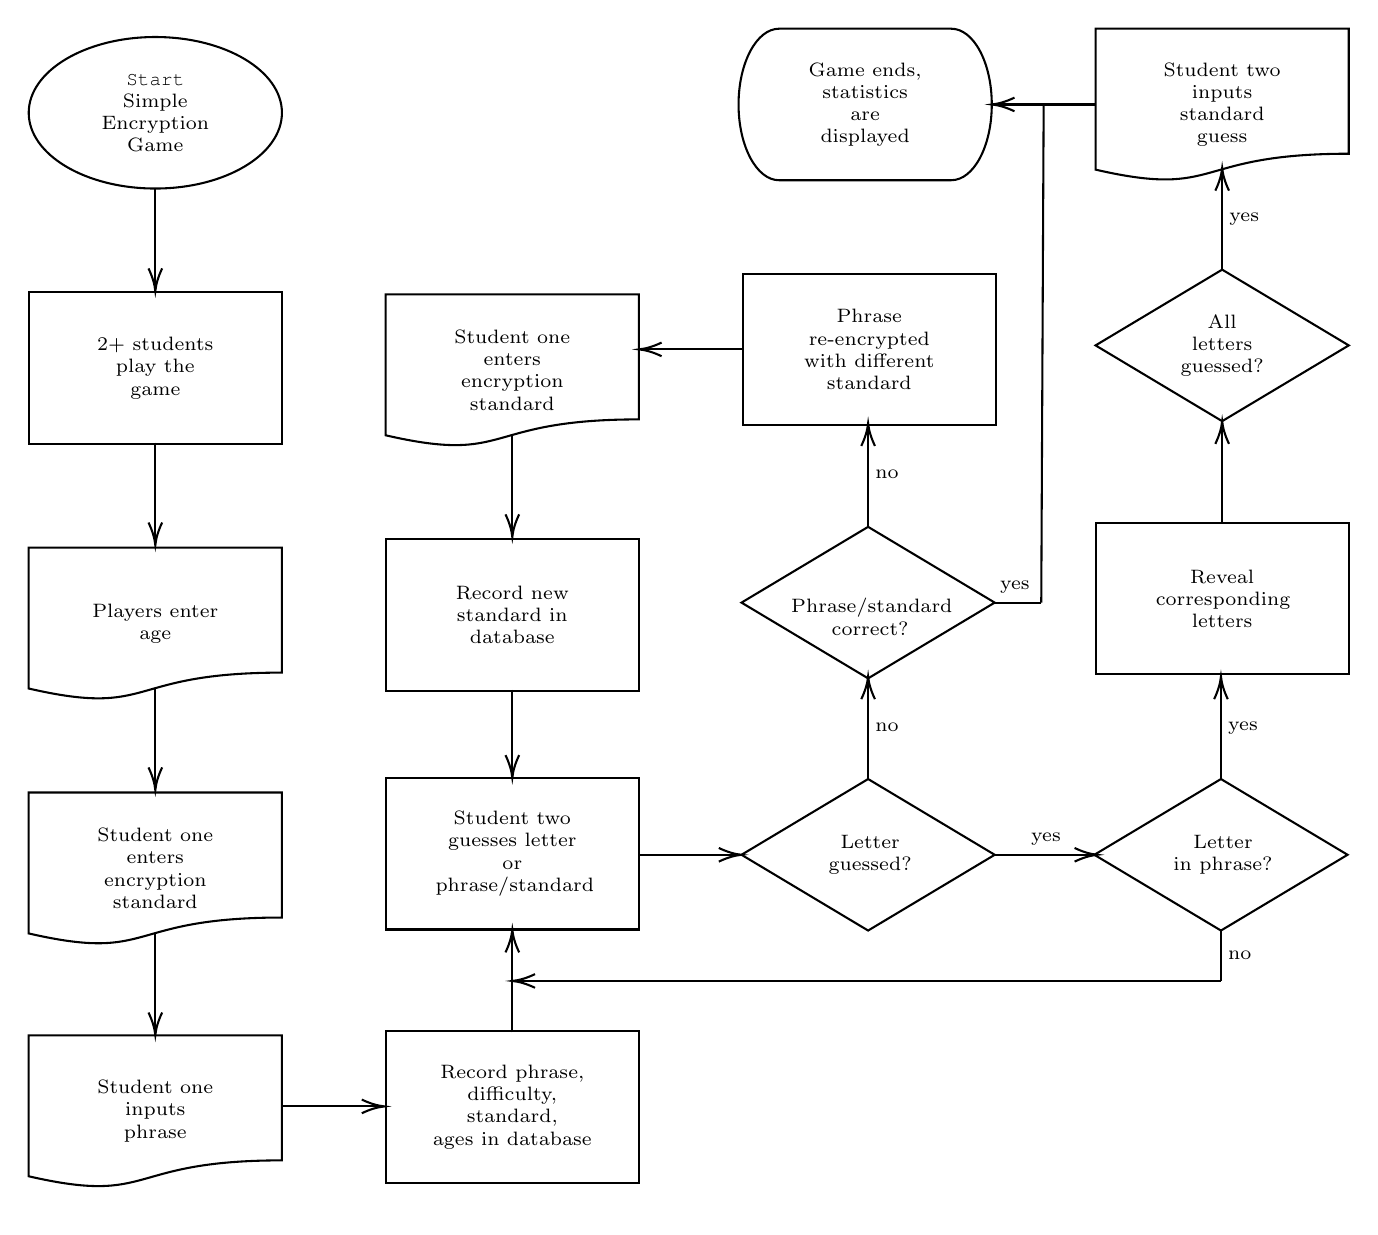
\begin{tikzpicture}[x=0.75pt,y=0.75pt,yscale=-1,xscale=1]
%uncomment if require: \path (0,582); %set diagram left start at 0, and has height of 582

%Shape: Ellipse [id:dp3892963566590173] 
\draw   (11,41.5) .. controls (11,21.34) and (38.31,5) .. (72,5) .. controls (105.69,5) and (133,21.34) .. (133,41.5) .. controls (133,61.66) and (105.69,78) .. (72,78) .. controls (38.31,78) and (11,61.66) .. (11,41.5) -- cycle ;
%Straight Lines [id:da19887855056316295] 
\draw    (72,78) -- (72,125.42) ;
\draw [shift={(72,127.42)}, rotate = 270] [color={rgb, 255:red, 0; green, 0; blue, 0 }  ][line width=0.75]    (10.93,-3.29) .. controls (6.95,-1.4) and (3.31,-0.3) .. (0,0) .. controls (3.31,0.3) and (6.95,1.4) .. (10.93,3.29)   ;
%Shape: Rectangle [id:dp014208133529669098] 
\draw   (11,128) -- (133,128) -- (133,201) -- (11,201) -- cycle ;
%Flowchart: Document [id:dp8688522724734018] 
\draw   (11,486) -- (133,486) -- (133,546.23) .. controls (56.75,546.23) and (72,567.94) .. (11,553.89) -- cycle ;
%Straight Lines [id:da5839938576291159] 
\draw    (72,200.42) -- (72,247.84) ;
\draw [shift={(72,249.84)}, rotate = 270] [color={rgb, 255:red, 0; green, 0; blue, 0 }  ][line width=0.75]    (10.93,-3.29) .. controls (6.95,-1.4) and (3.31,-0.3) .. (0,0) .. controls (3.31,0.3) and (6.95,1.4) .. (10.93,3.29)   ;
%Shape: Rectangle [id:dp912979444091131] 
\draw   (183,484) -- (305,484) -- (305,557) -- (183,557) -- cycle ;
%Straight Lines [id:da5083600057856885] 
\draw    (244,484.5) -- (244,437.08) ;
\draw [shift={(244,435.08)}, rotate = 90] [color={rgb, 255:red, 0; green, 0; blue, 0 }  ][line width=0.75]    (10.93,-3.29) .. controls (6.95,-1.4) and (3.31,-0.3) .. (0,0) .. controls (3.31,0.3) and (6.95,1.4) .. (10.93,3.29)   ;
%Straight Lines [id:da1366751880696635] 
\draw    (133,520.23) -- (180.42,520.23) ;
\draw [shift={(182.42,520.23)}, rotate = 180] [color={rgb, 255:red, 0; green, 0; blue, 0 }  ][line width=0.75]    (10.93,-3.29) .. controls (6.95,-1.4) and (3.31,-0.3) .. (0,0) .. controls (3.31,0.3) and (6.95,1.4) .. (10.93,3.29)   ;
%Shape: Rectangle [id:dp1281567774491723] 
\draw   (183,362) -- (305,362) -- (305,435) -- (183,435) -- cycle ;
%Shape: Boxed Line [id:dp041257977100174203] 
\draw    (305,399) -- (352.42,399) ;
\draw [shift={(354.42,399)}, rotate = 180] [color={rgb, 255:red, 0; green, 0; blue, 0 }  ][line width=0.75]    (10.93,-3.29) .. controls (6.95,-1.4) and (3.31,-0.3) .. (0,0) .. controls (3.31,0.3) and (6.95,1.4) .. (10.93,3.29)   ;
%Flowchart: Decision [id:dp6100652602081542] 
\draw   (415.42,362.5) -- (476.42,399) -- (415.42,435.5) -- (354.42,399) -- cycle ;
%Straight Lines [id:da2210516933251061] 
\draw    (415.42,362.5) -- (415.42,315.08) ;
\draw [shift={(415.42,313.08)}, rotate = 90] [color={rgb, 255:red, 0; green, 0; blue, 0 }  ][line width=0.75]    (10.93,-3.29) .. controls (6.95,-1.4) and (3.31,-0.3) .. (0,0) .. controls (3.31,0.3) and (6.95,1.4) .. (10.93,3.29)   ;
%Flowchart: Decision [id:dp5795837488593116] 
\draw   (415.42,241) -- (476.42,277.5) -- (415.42,314) -- (354.42,277.5) -- cycle ;
%Straight Lines [id:da8276046312641692] 
\draw    (415.42,240.5) -- (415.42,193.08) ;
\draw [shift={(415.42,191.08)}, rotate = 90] [color={rgb, 255:red, 0; green, 0; blue, 0 }  ][line width=0.75]    (10.93,-3.29) .. controls (6.95,-1.4) and (3.31,-0.3) .. (0,0) .. controls (3.31,0.3) and (6.95,1.4) .. (10.93,3.29)   ;
%Shape: Rectangle [id:dp40043316067990364] 
\draw   (355,119) -- (477,119) -- (477,192) -- (355,192) -- cycle ;
%Straight Lines [id:da00836568891618028] 
\draw    (476.42,399) -- (523.84,399) ;
\draw [shift={(525.84,399)}, rotate = 180] [color={rgb, 255:red, 0; green, 0; blue, 0 }  ][line width=0.75]    (10.93,-3.29) .. controls (6.95,-1.4) and (3.31,-0.3) .. (0,0) .. controls (3.31,0.3) and (6.95,1.4) .. (10.93,3.29)   ;
%Flowchart: Document [id:dp27877003106125287] 
\draw   (11,251) -- (133,251) -- (133,311.23) .. controls (56.75,311.23) and (72,332.94) .. (11,318.89) -- cycle ;
%Straight Lines [id:da9872348183315431] 
\draw    (72,318.42) -- (72,365.84) ;
\draw [shift={(72,367.84)}, rotate = 270] [color={rgb, 255:red, 0; green, 0; blue, 0 }  ][line width=0.75]    (10.93,-3.29) .. controls (6.95,-1.4) and (3.31,-0.3) .. (0,0) .. controls (3.31,0.3) and (6.95,1.4) .. (10.93,3.29)   ;
%Flowchart: Document [id:dp8293742293432909] 
\draw   (11,369) -- (133,369) -- (133,429.23) .. controls (56.75,429.23) and (72,450.94) .. (11,436.89) -- cycle ;
%Straight Lines [id:da33583291117449665] 
\draw    (72,436.5) -- (72,483.92) ;
\draw [shift={(72,485.92)}, rotate = 270] [color={rgb, 255:red, 0; green, 0; blue, 0 }  ][line width=0.75]    (10.93,-3.29) .. controls (6.95,-1.4) and (3.31,-0.3) .. (0,0) .. controls (3.31,0.3) and (6.95,1.4) .. (10.93,3.29)   ;
%Flowchart: Document [id:dp5517234599271172] 
\draw   (183,129) -- (305,129) -- (305,189.23) .. controls (228.75,189.23) and (244,210.94) .. (183,196.89) -- cycle ;
%Straight Lines [id:da11462356345116653] 
\draw    (244,196.5) -- (244,243.92) ;
\draw [shift={(244,245.92)}, rotate = 270] [color={rgb, 255:red, 0; green, 0; blue, 0 }  ][line width=0.75]    (10.93,-3.29) .. controls (6.95,-1.4) and (3.31,-0.3) .. (0,0) .. controls (3.31,0.3) and (6.95,1.4) .. (10.93,3.29)   ;
%Straight Lines [id:da2650692735370479] 
\draw    (355,155.5) -- (307,155.5) ;
\draw [shift={(305,155.5)}, rotate = 360] [color={rgb, 255:red, 0; green, 0; blue, 0 }  ][line width=0.75]    (10.93,-3.29) .. controls (6.95,-1.4) and (3.31,-0.3) .. (0,0) .. controls (3.31,0.3) and (6.95,1.4) .. (10.93,3.29)   ;
%Shape: Rectangle [id:dp6811663085657764] 
\draw   (183,247) -- (305,247) -- (305,320) -- (183,320) -- cycle ;
%Straight Lines [id:da7744902079092426] 
\draw    (244,319.5) -- (244,359.92) ;
\draw [shift={(244,361.92)}, rotate = 270] [color={rgb, 255:red, 0; green, 0; blue, 0 }  ][line width=0.75]    (10.93,-3.29) .. controls (6.95,-1.4) and (3.31,-0.3) .. (0,0) .. controls (3.31,0.3) and (6.95,1.4) .. (10.93,3.29)   ;
%Shape: Rectangle [id:dp6868092748581316] 
\draw   (525,239) -- (647,239) -- (647,312) -- (525,312) -- cycle ;
%Flowchart: Decision [id:dp07121461880236302] 
\draw   (585.42,362.5) -- (646.42,399) -- (585.42,435.5) -- (524.42,399) -- cycle ;
%Straight Lines [id:da05515754453210531] 
\draw    (585.42,459.79) -- (246,459.79) ;
\draw [shift={(244,459.79)}, rotate = 360] [color={rgb, 255:red, 0; green, 0; blue, 0 }  ][line width=0.75]    (10.93,-3.29) .. controls (6.95,-1.4) and (3.31,-0.3) .. (0,0) .. controls (3.31,0.3) and (6.95,1.4) .. (10.93,3.29)   ;
%Straight Lines [id:da41299779400165915] 
\draw    (585.42,435.5) -- (585.42,459.79) ;
%Straight Lines [id:da27670933317397006] 
\draw    (585.42,362.5) -- (585.42,315.08) ;
\draw [shift={(585.42,313.08)}, rotate = 90] [color={rgb, 255:red, 0; green, 0; blue, 0 }  ][line width=0.75]    (10.93,-3.29) .. controls (6.95,-1.4) and (3.31,-0.3) .. (0,0) .. controls (3.31,0.3) and (6.95,1.4) .. (10.93,3.29)   ;
%Flowchart: Decision [id:dp4806907963744267] 
\draw   (586,117.08) -- (647,153.58) -- (586,190.08) -- (525,153.58) -- cycle ;
%Straight Lines [id:da09784740458097874] 
\draw    (586,117.5) -- (586,70.08) ;
\draw [shift={(586,68.08)}, rotate = 90] [color={rgb, 255:red, 0; green, 0; blue, 0 }  ][line width=0.75]    (10.93,-3.29) .. controls (6.95,-1.4) and (3.31,-0.3) .. (0,0) .. controls (3.31,0.3) and (6.95,1.4) .. (10.93,3.29)   ;
%Straight Lines [id:da6080018155245943] 
\draw    (586,239.5) -- (586,192.08) ;
\draw [shift={(586,190.08)}, rotate = 90] [color={rgb, 255:red, 0; green, 0; blue, 0 }  ][line width=0.75]    (10.93,-3.29) .. controls (6.95,-1.4) and (3.31,-0.3) .. (0,0) .. controls (3.31,0.3) and (6.95,1.4) .. (10.93,3.29)   ;
%Straight Lines [id:da4919984780577087] 
\draw    (498.84,277.5) -- (476.42,277.5) ;
%Flowchart: Document [id:dp09854064656975048] 
\draw   (525,1) -- (647,1) -- (647,61.23) .. controls (570.75,61.23) and (586,82.94) .. (525,68.89) -- cycle ;
%Straight Lines [id:da6227975102616017] 
\draw    (525,37.5) -- (477,37.5) ;
\draw [shift={(475,37.5)}, rotate = 360] [color={rgb, 255:red, 0; green, 0; blue, 0 }  ][line width=0.75]    (10.93,-3.29) .. controls (6.95,-1.4) and (3.31,-0.3) .. (0,0) .. controls (3.31,0.3) and (6.95,1.4) .. (10.93,3.29)   ;
%Flowchart: Terminator [id:dp07962655437406885] 
\draw   (372.52,1) -- (455.48,1) .. controls (466.26,1) and (475,17.34) .. (475,37.5) .. controls (475,57.66) and (466.26,74) .. (455.48,74) -- (372.52,74) .. controls (361.74,74) and (353,57.66) .. (353,37.5) .. controls (353,17.34) and (361.74,1) .. (372.52,1) -- cycle ;
%Straight Lines [id:da9765378738053909] 
\draw    (500,37.5) -- (498.84,277.5) ;

% Text Node
\draw (72,41.5) node  [font=\scriptsize] [align=left] {\begin{minipage}[lt]{60.27pt}\setlength\topsep{0pt}
\begin{center}
{\fontfamily{pcr}\selectfont Start}\\Simple Encryption\\Game
\end{center}

\end{minipage}};
% Text Node
\draw (72,164.5) node  [font=\scriptsize] [align=left] {\begin{minipage}[lt]{47.58pt}\setlength\topsep{0pt}
\begin{center}
2+ students\\play the game
\end{center}

\end{minipage}};
% Text Node
\draw (72,522.5) node  [font=\scriptsize] [align=left] {\begin{minipage}[lt]{45.59pt}\setlength\topsep{0pt}
\begin{center}
Student one\\inputs phrase
\end{center}

\end{minipage}};
% Text Node
\draw (244,520.5) node  [font=\scriptsize] [align=left] {\begin{minipage}[lt]{61.59pt}\setlength\topsep{0pt}
\begin{center}
Record phrase,\\difficulty, standard,\\ages in database
\end{center}

\end{minipage}};
% Text Node
\draw (244,398.5) node  [font=\scriptsize] [align=left] {\begin{minipage}[lt]{55.51pt}\setlength\topsep{0pt}
\begin{center}
Student two\\guesses letter or\\phrase/standard
\end{center}

\end{minipage}};
% Text Node
\draw (416.42,399) node  [font=\scriptsize] [align=left] {\begin{minipage}[lt]{33.69pt}\setlength\topsep{0pt}
\begin{center}
Letter\\guessed?
\end{center}

\end{minipage}};
% Text Node
\draw (417.42,337.79) node [anchor=west] [inner sep=0.75pt]  [font=\scriptsize] [align=left] {no};
% Text Node
\draw (416.42,282.5) node  [font=\scriptsize] [align=left] {\begin{minipage}[lt]{57.1pt}\setlength\topsep{0pt}
\begin{center}
Phrase/standard \\correct?
\end{center}

\end{minipage}};
% Text Node
\draw (417.42,215.79) node [anchor=west] [inner sep=0.75pt]  [font=\scriptsize] [align=left] {no};
% Text Node
\draw (416,155.5) node  [font=\scriptsize] [align=left] {\begin{minipage}[lt]{67.42pt}\setlength\topsep{0pt}
\begin{center}
Phrase re-encrypted\\with different \\standard
\end{center}

\end{minipage}};
% Text Node
\draw (501.13,396) node [anchor=south] [inner sep=0.75pt]  [font=\scriptsize] [align=left] {yes};
% Text Node
\draw (72,287.5) node  [font=\scriptsize] [align=left] {\begin{minipage}[lt]{58.69pt}\setlength\topsep{0pt}
\begin{center}
Players enter age
\end{center}

\end{minipage}};
% Text Node
\draw (72,405.5) node  [font=\scriptsize] [align=left] {\begin{minipage}[lt]{57.49pt}\setlength\topsep{0pt}
\begin{center}
Student one\\enters encryption\\standard
\end{center}

\end{minipage}};
% Text Node
\draw (244,165.5) node  [font=\scriptsize] [align=left] {\begin{minipage}[lt]{57.49pt}\setlength\topsep{0pt}
\begin{center}
Student one\\enters encryption\\standard
\end{center}

\end{minipage}};
% Text Node
\draw (244,283.5) node  [font=\scriptsize] [align=left] {\begin{minipage}[lt]{40.82pt}\setlength\topsep{0pt}
\begin{center}
Record new\\standard in\\database
\end{center}

\end{minipage}};
% Text Node
\draw (586,275.5) node  [font=\scriptsize] [align=left] {\begin{minipage}[lt]{47.97pt}\setlength\topsep{0pt}
\begin{center}
Reveal\\corresponding\\letters
\end{center}

\end{minipage}};
% Text Node
\draw (586.42,399) node  [font=\scriptsize] [align=left] {\begin{minipage}[lt]{36.07pt}\setlength\topsep{0pt}
\begin{center}
Letter\\in phrase?
\end{center}

\end{minipage}};
% Text Node
\draw (587.42,447.64) node [anchor=west] [inner sep=0.75pt]  [font=\scriptsize] [align=left] {no};
% Text Node
\draw (587.42,337.79) node [anchor=west] [inner sep=0.75pt]  [font=\scriptsize] [align=left] {yes};
% Text Node
\draw (586,153.58) node  [font=\scriptsize] [align=left] {\begin{minipage}[lt]{33.69pt}\setlength\topsep{0pt}
\begin{center}
All letters\\guessed?
\end{center}

\end{minipage}};
% Text Node
\draw (588,92.79) node [anchor=west] [inner sep=0.75pt]  [font=\scriptsize] [align=left] {yes};
% Text Node
\draw (486.13,274.5) node [anchor=south] [inner sep=0.75pt]  [font=\scriptsize] [align=left] {yes};
% Text Node
\draw (586,37.5) node  [font=\scriptsize] [align=left] {\begin{minipage}[lt]{51.55pt}\setlength\topsep{0pt}
\begin{center}
Student two\\inputs standard\\guess
\end{center}

\end{minipage}};
% Text Node
\draw (414,37.5) node  [font=\scriptsize] [align=left] {\begin{minipage}[lt]{42.4pt}\setlength\topsep{0pt}
\begin{center}
Game ends,\\statistics are\\displayed
\end{center}

\end{minipage}};


\end{tikzpicture}
